\documentclass[a4paper,12pt]{article}
\usepackage[T1]{fontenc}
\PassOptionsToPackage{defaults=hu-min}{magyar.ldf}
\usepackage[magyar]{babel}
\usepackage[a4paper]{geometry}
\geometry{margin=2cm}
\usepackage{graphicx}
\usepackage{fancyhdr}



\pagestyle{fancy}
\fancyhf{}
\fancyhead[LE,RO]{\normalfont\normalsize\thepage}
\fancyhead[RE]{\nouppercase{\sffamily\small\leftmark}}
\fancyhead[LO]{\nouppercase{\sffamily\small\rightmark}}


\begin{document}
\title{\textsc{Webprogramozás III. Gy. \\ {\normalsize (LBT\_IM744G2)}} \\ {\normalsize Beadandó feladat dokumentáció}}
\author{Kovács Norbert \\ ANOXWJ}
\maketitle
\newpage
\tableofcontents
\newpage


\section{Weboldal koncepciója}

\textbf{Github link:}
\begin{center}
\textit{	https://github.com/Gellifree/bluepaw.git}
\end{center}

\subsection{Technikai részletek}
A beadandó feladatot, az órán is alkalmazott \textit{xampp} szerverrel kívánom megvalósítani, \textit{apache netbeans} fejlesztőkörnyezettel. A Mysql kezelését a videóban is használt, \textit{phpmyadmin} oldalon intézem. Nem fontos részlet, a megvalósítás szempontjából, de a Windows operációs rendszer, virtuális gépként fut.

\begin{center}
	\textit{{\footnotesize Követelmény: ,,A beadandó feladat PHP MVC keretrendszerben készül!''}}
\end{center}

\begin{itemize}
	\item OS: Windows 10 Pro (21H1)
	\item Kernel: 10.0.19041.1023
	\item Mysql: 10.4.19-MariaDB
	\item PHP: 8.0.6
	\item Apache Netbeans IDE: 12.3
	\item CodeIgniter: 3.1.11
\end{itemize}

\subsection{Elképzelés}
A weboldal egy \textit{fiktív} szervezet köré épül, aminek a feladata  az \textit{állategészségügy}, és \textit{állatvédelem}. A fiktív szervezetnek több városban lesznek épületei országszerte. Egy városban több különféle épület is tartozhat a szervezethez. Például tartozhat állatmenhely, ahol kutyákat tárolnak, állatorvosi rendelő vagy éppen raktárépület.

Hasonlóképpen az egyetemi példafeladathoz, ahol
\begin{center}
	Kampusz -> Épület -> Terem \\[0.5cm]
	Pl.: Eger -> C épület -> 124-es terem,
\end{center}
felosztás található, itt is három rétegre kívánom felosztani a problémát, mégpedig:
\begin{center}
	Régió -> Épület -> Iroda\\[0.5cm]
	Pl.: Miskolc -> Orvosi rendelő -> 1-es vizsgáló
\end{center}

A fiktív szervezetet, az előző beadandóm állatotthonából fejlesztem tovább, részben idő spórolás céljából, részben a hasonló koncepcióból adódóan.\\
Szervezet neve: \textbf{Kék mancs}.


\section{Adatbázis tervezése}
Az adatbázis során a következőkben tervezett entitásokon kívül, még számos entitással lehetne bővíteni az adatbázist, viszont így is 7 tábla születik, a kapcsoló tábla figyelembe vétele nélkül.


\subsection{ER modell}
A pluszba kapott egyedi azonosító mezőket, és az idegen kulcsokat nem tüntetjük fel a tervezés során.

\begin{enumerate}
	\item Régió \\
	Egy Régió eltárolásához, elegendő a régió \textit{neve} (ami gyakorlatilag a város neve), és egy \textit{leírás} mező.
	
	\item Épület \\
	Az épület entitás kapcsán, elég tárolnunk az épület \textit{nevét}, és \textit{leírását}.
	
	\item Iroda \\
	Egy épület alegysége, az iroda entitás lesz. Elegendő tárolnunk a \textit{nevét}, és a \textit{kapacitását}.
	
	\item Kutya \\
	Egy kutya esetén, tárolnunk kell a \textit{nevét}, \textit{leírását}, \textit{születési évét}, \textit{nemét} és egy hozzá tartozó \textit{képet}. A kutya \textit{életkora}, származtatott tulajdonság lesz.
	
	\item Alkalmazott \\
	Az alkalmazottak esetén, tároljuk el az alkalmazott teljes \textit{nevét}.
	
	\item Feladatkör \\
	A feladatkörnek \textit{tároljuk} a nevét és \textit{leírását}.
	
	\item Munkakör \\
	A munkakör kapcsán, tároljuk a \textit{nevét}, a \textit{leírását}, és a hozzá tartozó \textit{fizetést}.
\end{enumerate}

\begin{center}
	\includegraphics[width = 17cm]{"draw_io/SQL_tervezés.png"} \\
	{\small Az ER modell}
\end{center}

\begin{center}
	\textit{{\small Követelmény: ,,A megvalósítandó projekthez tartozó adatmodell legalább 5 forgalmi adattáblát tartalmaz (a külső modulok által használt táblákon kívül). Az adatmodell legalább 3. normálformában van és modellben megtalálható az egy-több, valamint a több-több típusú kapcsolat is. A technikai okokból létrehozott táblák (kapcsolótáblák) nem tekintendőek forgalmi táblának.''}}
\end{center}
\newpage
\subsection{Relációs adatmodell}
Az elkészült modell alapján, a következő táblák jöttek létre.
\begin{center}
	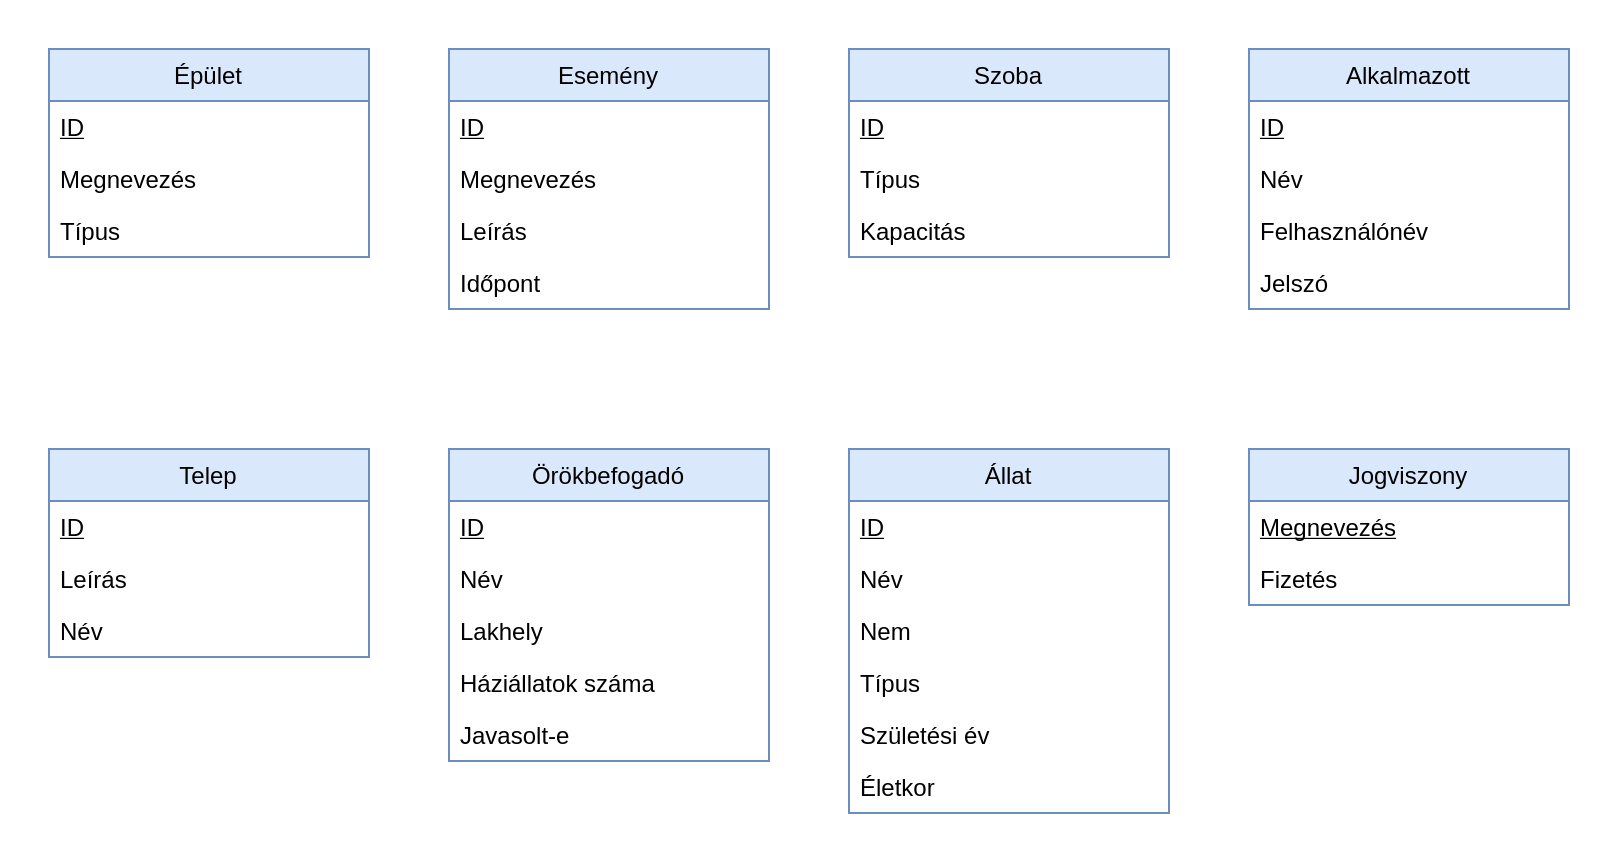
\includegraphics[width = 15cm]{"draw_io/SQL_Táblák.png"} \\
	{\small Az ER modell}
\end{center}
Hozzuk létre a szükséges kapcsolótáblákat, és illesszük be az idegen kulcsokat, majd jelöljük a kapcsolatokat.

\begin{center}
	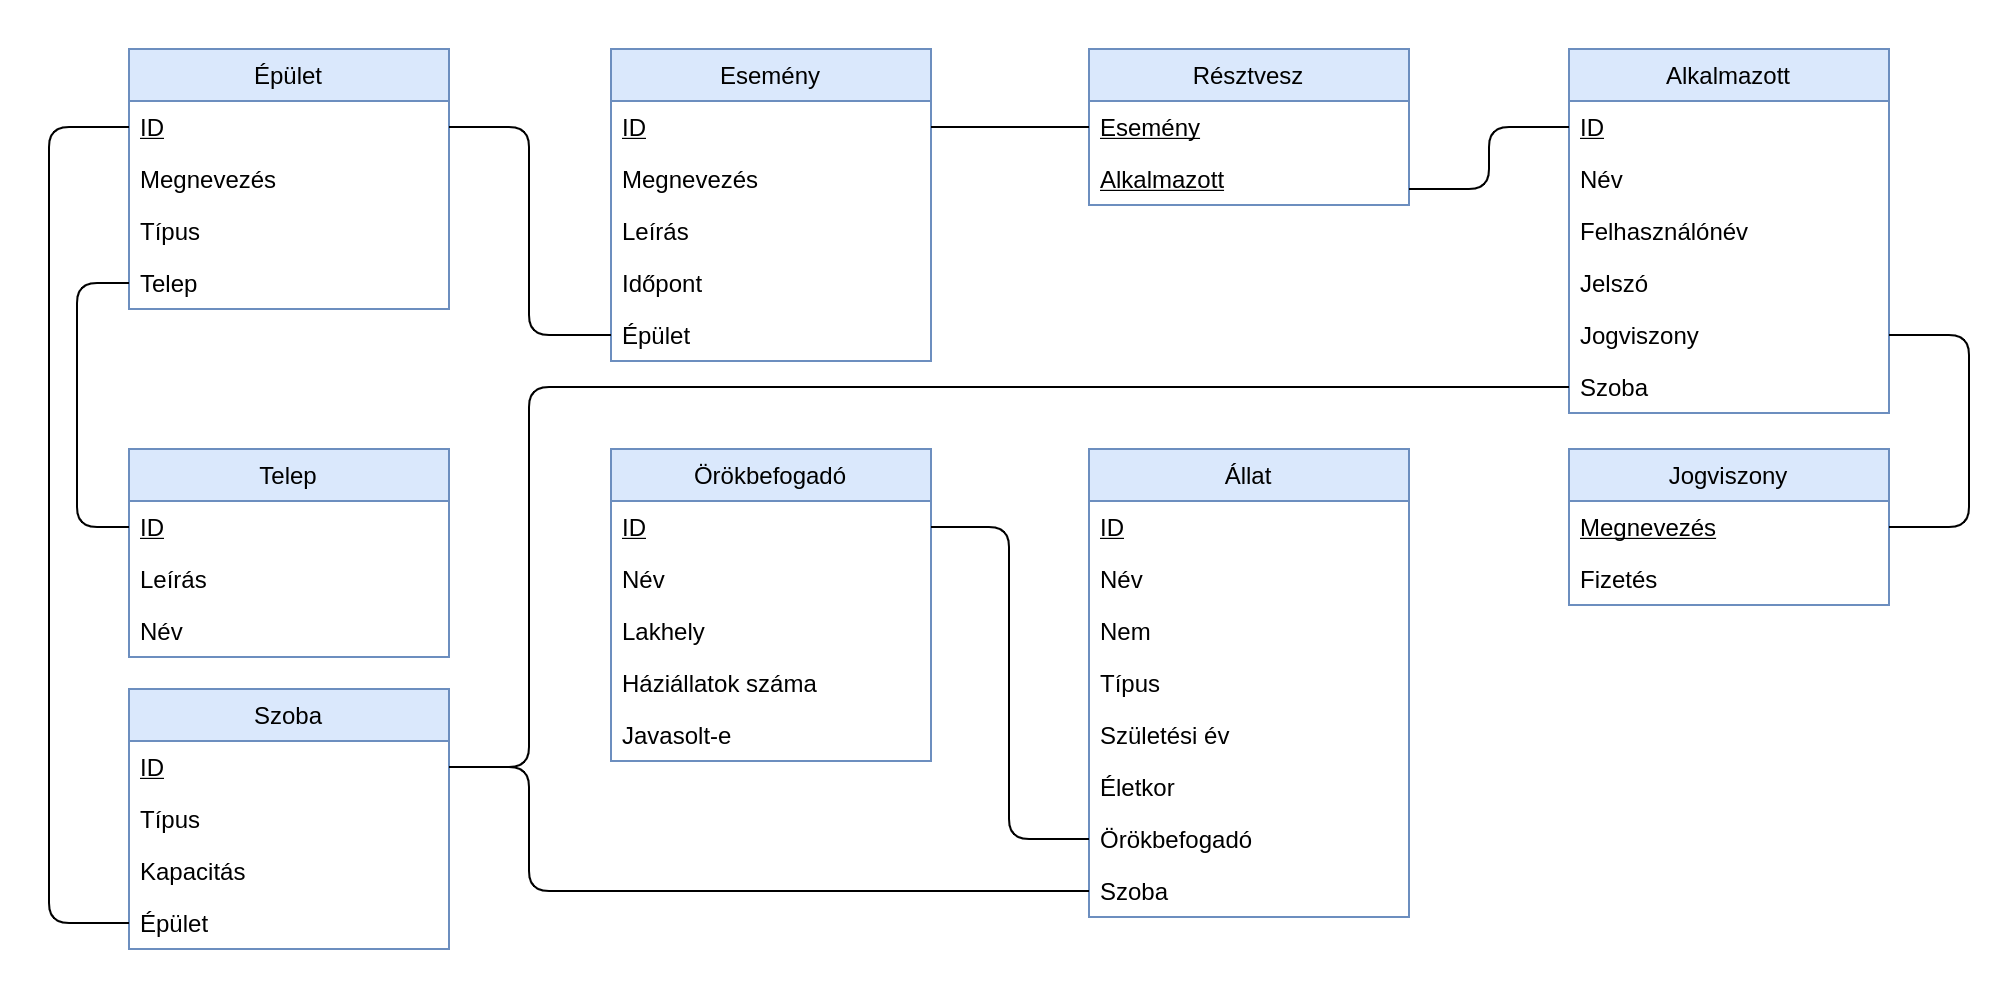
\includegraphics[width = 18cm]{"draw_io/SQL_Táblák_kapcsolatok.png"} \\
	{\small Az ER modell a kapcsolatokkal}
\end{center}
\subsection{SQL parancsok}
Az \textit{SQL} parancsok megtalálhatóak az \textit{application/create.sql} fájlban. Ebben, minden \textit{SQL} parancs megtalálható, amit manuálisan futtattunk a \textit{phpmyadmin} oldalon keresztül. A végleges adatok természetesen már nem \textit{SQL} parancsokkal kerültek fel a weboldalra, hanem a grafikus felületen keresztül, így azok itt nem rögzítettek.
\section{Összefoglaló}
Összességében, a projekt sok hiányossággal rendelkezik. A követelményekből, a fájl feltöltés, megvalósításra került, és integrálva lett, a fájlok letöltésének funkciója, ugyan technikailag megtalálható a projekt forrásállományai között, az semmilyen formában nem lett integrálva a weboldallal, és nem használható, így ez nem tekinthető megvalósítottnak.

A nézetek reszponzívak ugyan, de a táblázatok eseténél a reszponzivitás nagyon kis ablakméretnél megtörhet.

A csoportkezelés technikailag megvalósul, és minden Controller eseténél megtalálható a csoport ellenőrzése, a megfelelő műveleteknél. Általánosan kifejezve a \textit{Controller} nevét követi a \textit{manager} kifejezés.

A gyakorlatban még számos egyéb kényelmi probléma vetül fel. Egy adott munkakörhöz hozzálehet rendelni bármennyi feladatkört, és ellenőrizve is vannak, egyedi validációs függvénnyel a duplikációk, de a felületen, nincs átadva a hozzáadó nézetnek, a munkakör azonosítója, így azt is ki kell választani, amikor feladatkört rendelünk hozzá. Ez kifejezetten kényelmetlen, és megoldásra szorulna, a munkakor paraméterének átadásával.

Az adatbázis felépítése során úgy építettük fel az adatokat, hogy egy alkalmazott egy irodához, nem épülethez rendelt. Ez alapesetben rendben is volna, egészen addig, amíg nem olyan munkakörről van szó, ami nem értelmezhető csak irodára. Például egy takarító alkalmazottat, nem irodához kellene értelmeznünk, hanem épülethez. Bizonyos munkakörök esetében, viszont az iroda megközelítés áll helyt, pl egy adminisztrátori munkakörben. Ennek feloldásához valószínűleg újra kellene tervezni az adatbázist.

Ezenkívül praktikus volna, különféle lekérdezéseket megvalósítani, a listázó nézetek praktikusabbá tétele érdekében. A szűrés funkciója, miszerint egy adott tulajdonság alapján szűrjünk, kifejezetten hasznos lenne. Pl csak azokat az épületeket listázza ki, amik egy adott régióhoz tartoznak.

Ezenkívül, egy egyedi rendezési szempont elkészítése is hasznos lenne. Miszerint, a listázó nézet, valamilyen oszlop alapján rendezett, és ezt a felhasználó változtathatja. Ezt véleményem szerint, úgy lehetne megoldani, hogy a listázó nézetet, elválasztom az egyedi nézettől, és a listázó nézet paraméterét, a rendezés szempontjaként értelmezném. Ezáltal, a megfelelő helyre, a megfelelő id-vel rendelkező linkek alapján, át tudnánk adni a modellen keresztül egy olyan lekérdezést, ahol a rendezés szempontja, a paraméterben kapott mező. Természetesen ebben az esetben, az egyedi nézethez rendelnünk kell egy új függvényt. 


\end{document}
